
%Chapter 8
 
\chapter{Sequences and Series}



\section{General Sequences}\begin{enumerate}


\item How do you recognize geometric sequences?  Determine a sure fire and easy-to-remember method for finding a formula for any geometric sequence.  Explain how to use your method.

\item Are all convergent sequences alike?  Describe the possible behavior of convergent sequences.

\item The limit of a sequence that is monotonic and bounded must exist, but without some other tools we do not know what the value of the limit is.  Where else have we seen theorems that tell us that something exists but do not directly give us a way to find that value?  Why are these theorems, called existence theorems, useful?

\item To determine if a sequence converges sometimes we find a limit as $n \rightarrow  \infty$.  Describe the tools in your limit toolkit that will help you find these limits.

\item Technically, the sequences $
\left\{ {a_n } \right\}$  we are working with are not continuous functions, but we use the theorems we learned for continuous functions to find the limits of these functions.  Doesn't this violate everything that was ever said about checking the hypotheses before using a theorem?  Comments.

\item Why does L'Hospital's Rule technically not apply to limits of sequences?  Why can we use it anyway?

\item Previously we looked at limits of continuous (and sometimes not continuous) functions.  Now we are studying limits of discrete functions.  Compare and contrast the 2 concepts.

\item Create a concept map of the tools you know of for sequence convergence that will help you understand when and in what order to apply these tests.

\item Compare and contrast 2 ways to plot a sequence.  Which plot do you prefer?  What limitations do these plots have?

\item True or false: : If $a_n > 0$ for all $n$ and $a_n  \to L$, then $L > 0$.	

\item True or false: : If $a_n = 0$ for all $n$ and $a_n  \to L$, then $L = 0$.

\item True or false: If $a_n > 0$ for all $n$ and $\left( { - 1} \right)^n a_n  \to L$, then $L = 0$.

\item Suppose I know that $
\left\{ {a_n } \right\}_{n = 1}^\infty   \to L$.  What do I know about $\left\{ {a_n } \right\}_{n = 4}^\infty  $?

\item How do you recognize an arithmetic?  Determine an easy-to-remember method for finding the formula for any arithmetic sequence.  Explain how to use your method.

\end{enumerate}\section{Divergent and Oscillating Sequences}\begin{enumerate}

\item Are all divergent sequences alike?  Describe the possible behavior of sequences.

\item A sequence might diverge because of oscillation.  Explain what we mean by this.  Does every sequence that oscillates diverge?

\item A sequence is said to diverge if it does not converge.  The word "diverge" is well chosen for sequences that diverge to 8, but is less descriptive of sequences such as $
\left\{ {1,\,\,2,\,\,1,\,\,2,\,\,1,\,\,2,\,\, \ldots } \right\}$ and $\left\{ {1,\,\,2,\,\,3,\,\,1,\,\,2,\,\,3,\,\, \ldots } \right\}$.  Describe the limiting behavior of these sequences and discuss other possible limiting behaviors of divergent sequences.  \cite{SM}

\item Since we know $
\mathop {\lim }\limits_{x \to \infty } \frac{1}{{x^2 }} = 0$, we can conclude $
\mathop {\lim }\limits_{k \to \infty } \frac{1}{{k^2 }} = 0$.  When can we draw conclusions about $
\mathop {\lim }\limits_{k \to \infty } a_k $ from the limit of a corresponding continuous function and when can we not?

\item Compare and contrast $
\mathop {\lim }\limits_{x \to \infty } \sin \pi x$ and $
\mathop {\lim }\limits_{n \to \infty } \sin \pi n$.  \cite{SM}

\end{enumerate}\section{Monotonicity, Boundedness and Sequences}\begin{enumerate}

\item A sequence that is monotonic and bounded must converge.  Are both of these conditions necessary?  If so, find counterexamples to show they are necessary.  How can we check for monotonicity?

\item Determine whether each of the following scenarios describes a convergent sequence, a divergent sequence, or is inconclusive.  Justify your answers.
Monotonic increasing	Monotonic decreasing

\item A sequence that is monotonic and bounded must converge.  What if a sequence is only monotonic beyond a certain point?  In other words, what if for $
\left\{ {a_n } \right\}_{n = 1}^\infty  $ the values of $a_i$ oscillate until $n = 100$ and are monotonic for all $n > 100$?

\item A sequence that is monotonic and bounded must converge.  If a sequence is bounded and converges, is it monotonic?  If a sequence is monotonic and converges, is it bounded?

\item True or false: If $
\left\{ {a_n } \right\}$ is bounded, then $\left\{ {a_n } \right\}$ converges.	

\item True or false: If $\left\{ {a_n } \right\}$ is not bounded, then $\left\{ {a_n } \right\}$ diverges.

\item True or false: If $
\left\{ {a_n } \right\}$ is decreasing, then $\left\{ {a_n } \right\}$ converges.

\item True or false:  If $\left\{ {a_n } \right\}$ is decreasing and $a_n > 0$ for all  $n$, then $\left\{ {a_n } \right\}$ converges.

\item True or false: If $
\left\{ {a_n } \right\}$ is neither increasing nor decreasing, then $\left\{ {a_n } \right\}$diverges.

\item Consider this test: If $a_{n + 1}  - a_n  > 0$ for all $n$, then $
\left\{ {a_n } \right\}$ is strictly increasing.  Explain why the test works and apply it to $\left\{ {\frac{1}{n}} \right\}
$.  Create a similar test for strictly decreasing.

\item Consider this test: If $
\frac{{a_{n + 1} }}{{a_n }} > 1$ for all $n$, then $\left\{ {a_n } \right\}$ is strictly increasing.  Explain why the test works and apply it to $
\left\{ {\frac{1}{n}} \right\}$.  Create a similar test for nonincreasing.

\item Consider this test: Let $y = f(x)$ such that $
a_n  = f(n)$, and if $f'\left( x \right) > 0$ for all $x = 1$, then $\left\{ {a_n } \right\}$ is strictly increasing.  Explain why the test works and apply it to $\left\{ {\frac{1}{n}} \right\}$.  Create a similar test for nondecreasing.

\item Create a concept map of the following terms:  increasing, decreasing, strictly increasing, strictly decreasing, nonincreasing, nondecreasing and monotonic.  Give examples to supplement your concept map.

\end{enumerate}\section{General Series}\begin{enumerate}

\item Sometimes we can decide whether a series converges without knowing what the series converges to.  In a way this seems like cheating - it's like saying you know the answer exists but you don't know what it is - and it's okay not to know!  Explain the difference between knowing that a series converges and knowing what it converges to.  Make a convincing argument that shows why this is possible.

\item Create an infinite series of nonzero terms whose sum is 1, another series whose sum is $-3$ and a third whose sum is 0.  Can you create an infinite series of nonzero terms that converges to any given number?  How?  \cite{FWG}

\item The word "series" means a lot of things in everyday language that are not consistent with the mathematical language.  Knowing the specific meaning of the words associated with sequences and series are important.  Define and illustrate (possible compare and contrast) each of the following:  sequence, series, $n$th term, and partial sum.

\item Consider adding a finite number of terms to a convergent series.  What does this mean and how do we show this notionally?  Can the addition of a finite number of terms cause the series to diverge?  Consider adding a finite number of terms to a divergent series.  Can the addition of a finite number of terms cause the series to converge?

\item Compare and contrast these 2 statements.  \begin{enumerate} \item If $\sum _{n = 1}^\infty  {a_n } $ converges, then $a_n  \to 0$.                       \item If $a_n  \to 0$ , then $\sum _{n = 1}^\infty  {a_n } $ converges.\end{enumerate}

\item Can you obtain a convergent series by combining divergent series?  \cite{EP}

\item Can we obtain a divergent series by combining convergent series?

\item Compare and contrast the convergence and divergence of sequences and series.

\item List and describe a variety of applications that result in a sequence (but not in a series).  List and describe a variety of applications that result in a series.

\item True or false: If $\displaystyle\sum _{n = 1}^\infty  {a_n } $ and $\displaystyle\sum _{n = 1}^\infty  {b_n } $ diverge, then $
\displaystyle\sum _{n = 1}^\infty  {\left( {a_n  + b_n } \right)} $ diverges.

\item True or false: If $
\displaystyle\sum _{n = 1}^\infty  {a_n } $ converges and $\displaystyle\sum _{n = 1}^\infty  {b_n } $ diverges, then $\displaystyle\sum _{n = 1}^\infty  {\left( {a_n  + b_n } \right)} $ diverges.

\item True or false: If $\left\{ {a_n } \right\}$ is monotonic and bounded, then $\displaystyle\sum _{n = 1}^\infty  {a_n } $ converges.

\item True or false: If $\displaystyle\sum _{n = 1}^\infty  {a_n } $ and$\displaystyle\sum _{n = 1}^\infty  {b_n } $ converge, then $\displaystyle\sum\limits_{n = 1}^\infty  {\left( {a_n b_n } \right)}  = \left( {\displaystyle\sum\limits_{n = 1}^\infty  {a_n } } \right)\left( {\displaystyle\sum\limits_{n =1}^\infty  {b_n } } \right)$.

\item True or false: If $\displaystyle\sum _{n = 1}^\infty  {\left( {a_n } \right)^2 } $ and converges, then $\displaystyle\sum _{n = 1}^\infty  {a_n } 
$ converges.

\item True or false: If $\displaystyle\sum _{n = 1}^\infty  {a_n } $ and converges, then $\displaystyle\sum _{n = 1}^\infty  {\left( {a_n } \right)^2 } $ converges.

\item Suppose I know that $\displaystyle\sum _{n = 1}^\infty  {a_n } $
 converges to $K$.  What do I know about $\displaystyle\sum _{n = 4}^\infty  {a_n } $?

\item Determine the convergence of these series.  \begin{enumerate}\item $\displaystyle\sum\limits_{n = 0}^\infty  {\frac{{n^3 }}{{3^n }}} $	\item $\displaystyle\sum\limits_{n = 0}^\infty  {\frac{{n^3 }}{{n!}}} $	\item $\displaystyle\sum\limits_{n = 0}^\infty  {\frac{{n!}}{{3^n }}} $
\end{enumerate}

What do your results tell you about the relative growth rate of $f(x) = x!$, $f(x) = 3^x$ and $f(x) = x^3$?  Use you conjecture to determine the convergence of these series by inspection.
 	 	 
 	 	 	

\item Investigate the validity of this statement:  $
\displaystyle\sum\limits_{n = 1}^\infty  {\frac{1}{n}}  = \frac{\pi }{6}$.

\item Investigate the validity of this statement:  $
\displaystyle\sum\limits_{n = 2}^\infty  {\frac{1}{{n^2  - n}}}  = 1$.

\item Investigate the validity of this statement:  $
\displaystyle\sum\limits_{n = 1}^\infty  {\frac{1}{{n^2 }}}  = \frac{{\pi ^2 }}{6}$.

\item Investigate the validity of this statement:  $
\displaystyle\sum\limits_{n = 1}^\infty  {\frac{{\left( { - 1} \right)^n }}{n}}  = \frac{3}{4}$.

\end{enumerate}\section{Partial Sums}\begin{enumerate}

\item Consider the series $\displaystyle\sum\limits_{k = 1}^\infty  {a_k } $ and the 2 limits $\mathop {\lim }\limits_{k \to \infty } a_k $ and $\mathop {\lim }\limits_{k \to \infty } s_k $ where $s_k  = a_1  + a_2  +  \cdots  + a_k $.  Explain what these limits are and how they are related to each other.  Describe what you know about the series based on the results of the limits.  Can you conclude anything about one of the limits given the results of the other?

\item True or false: If the partial sums of $
\displaystyle\sum _{n = 1}^\infty  {a_n } $ are bounded, then $\displaystyle\sum _{n = 1}^\infty  {a_n } $ converges.

\item True or false: If $a_n = 0$ and the partial sums of $
\displaystyle\sum _{n = 1}^\infty  {a_n } $ are bounded, then $\displaystyle\sum _{n = 1}^\infty  {a_n } $ converges.

\item Explain in what ways determining the convergence of a series is simply the same as determining the convergence of a sequence.  When is this a useful idea?  When is this not a useful idea?

\item Prove that $
\displaystyle\sum\limits_{n = 1}^\infty  n $ diverges by using the fact that $\displaystyle\sum\limits_{n = 1}^k n  = \frac{{k\left( {k + 1} \right)}}{2}$.  Now, find another way to prove this series diverges.

\end{enumerate}
\section{Divergence Test}
\begin{enumerate}

\item Explain how to use the Divergence Test and give an explanation of why it works.  Why is the converse of the Divergence Test not true?

\item If $
\displaystyle\sum _{n = 1}^\infty  {a_n }  = L$ and $L$ is finite, what can we say about $
\mathop {\lim }\limits_{x \to \infty } a_n $?

\item If $\mathop {\lim }\limits_{x \to \infty } a_n  = L$
 and $L$ is finite, what can we say about $\displaystyle\sum _{n = 1}^\infty  {a_n } $?

\item True or false:  If $a_n $ converges then $\displaystyle\sum _{n = 1}^\infty  {a_n } $ converges.

\item True or false:  If $\displaystyle\sum _{n = 1}^\infty  {a_n } $ converges then $a_n $ converges.

\end{enumerate}
\section{Geometric Series}
\begin{enumerate}

\item True or false: $
\displaystyle\sum\limits_{k = 0}^\infty  {x^k }  = \frac{1}{{1 - x}}$ whenever $x \ne 1$.

\item Compare and contrast the convergence of geometric series and geometric sequences.

\item We know that $\displaystyle\sum\limits_{n = 0}^\infty  {ar^n }  = \frac{a}{{1 - r}}$ when $\left| r \right| < 1$.  Suppose $r$ is a specific positive value between 0 and 1.  How does the value of $\displaystyle\sum\limits_{n = 0}^\infty  {ar^n }$ compare to $\displaystyle\sum\limits_{n = 0}^\infty  {a\left( { - r} \right)^n } $?  Reconcile your results of the closed form formula with what is happening in the sum.

\item How do you recognize geometric series?  Determine a sure fire and easy-to-remember method for finding a formula for any geometric series.  Explain how to use your method.

\item We know that $
\displaystyle\sum\limits_{n = 0}^\infty  {ar^n }  = \frac{a}{{1 - r}}$ for specific values of $r$.   How do you find $\displaystyle\sum\limits_{n = 3}^\infty  {ar^n } $?  Find a general formula for $\displaystyle\sum\limits_{n = k}^\infty  {ar^n } $ when this series converges.

\item What is the general form of a geometric series?  How do we find the convergence of geometric series?  Using a picture and a specific convergent geometric series, show what it means for the series to converge.  How might geometric series show up in "real life"?

\item We know that if a geometric series converges, it converges to $
\frac{a}{{1 - r}}$
.  A friend of yours missed class when we went over geometric series and doesn't know how to find a and r.  Explain in words what these 2 parameters are and how to find them from a series.  Be sure to show an example where the geometric series is written in summation notation and another example when the terms are written out in a sum.

\item In one throw of two dice, the probability of getting a roll of 7 is $
p = \frac{1}{6}$.  If you throw the dice repeatedly, the probability that a 7 will appear for the first time at the nth throw is $
pq^{n - 1} $, where $q = 1 - p = \frac{5}{6}$.  Explain how this was calculated.  The expected number of throws until a 7 first appears is $
\displaystyle\sum\limits_{n = 1}^\infty  {npq^{n - 1} } $.  (You may have to look up the definition of expected values in a statistics book.)  Find the expected number of throws.  \cite{FWG}  Repeat this to find the expected number of throws before you get a 2.  Observations?

\item Suppose a bug starts at the origin of a 2-dimensional coordinate system and begins a little walk.  First it walks 1 unit up.  Then 0.5 units left.  Then 0.25 units down.  Then 0.125 units right.  It continues in this fashion, making a right turn after walking half the distance since its previous turn.  To what point does the bug converge?  \cite{SBS}

\item Use geometric series to find the fractional representation 0.333333... .  Use geometric series to find the fractional representation of 0.9999... .  Observations?

\item Consider a piece of paper represented in Figure \ref{ThirdEqualHalf}.  We are going to create 2 piles of paper bits.  In Step 1,  we cut the paper into thirds and one-third in each of Pile 1 and Pile 2.  In Step 2, we repeat the process.  Continue forever.  Explain the connection between this process and the sum 
$$\sum_{n=0}^\infty {1\over 3^n} = 2.$$

\begin{figure}[ht]
	\centering
		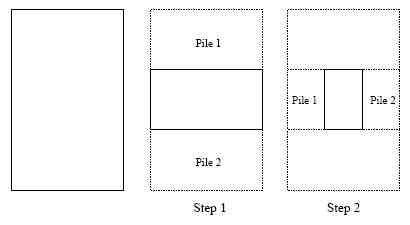
\includegraphics{TeXGraphics/Chapter8Fig.jpg}
	\caption{Tearing paper into thirds to make two piles.}
	\label{ThirdEqualHalf}
\end{figure}

\item Consider Zeno's paradox (refer to the text for details).  Assume that it takes a runner $\frac{1}{2}$ hour to run the first $\frac{1}{2}$
 of the course.  How long would it take the runner to complete the course?  Describe a situation, in the context of the paradox, in which it would take the runner an infinite amount of time to complete the course.

\item Figure \ref{GeoSeries1} gives an informal proof that $
\displaystyle\sum\limits_{n = 1}^\infty  {\frac{1}{{2^n }}}  = 1$.  Explain what is going on.

\begin{figure}[ht]
	\centering
		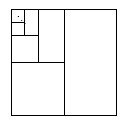
\includegraphics{TeXGraphics/GeoSeries1.jpg}
	\caption{$\displaystyle\sum\limits_{n = 1}^\infty  {\frac{1}{{2^n }}}  = 1$}
	\label{GeoSeries1}
\end{figure}

\item Figure \ref{GeoSeries2} gives an informal proof that $\displaystyle\sum\limits_{n = 1}^\infty  {\frac{3}{{4^n }}}  = 1$.  Explain what is going on. %insert file GeoSeries2.bmp or whatever at this point%
\begin{figure}[ht]
	\centering
		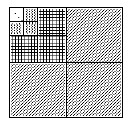
\includegraphics{TeXGraphics/GeoSeries2.jpg}
	\caption{$\displaystyle\sum\limits_{n = 1}^\infty  {\frac{3}{{4^n }}}  = 1$}
	\label{GeoSeries2}
\end{figure}

\end{enumerate}
\section{$p$-series}
\begin{enumerate}

\item If there were something called a $p$-sequence, what would it be?  Compare and contrast the convergence of $p$-series and $p$-sequences.

\item What is a $p$-series?  When do $p$-series converge and when do they diverge?  What tests can we use to verify these results?  

\item If there were something called a $p$-sequence, what would it be?  If there were something called an alternating $p$-series, what would it be?  Compare and contrast the convergence of $p$-series, alternating $p$-series, $p$-sequences and alternating $p$-sequences.

\item Compare and contrast the $p$-series and the $q$-log series.

\end{enumerate}
\section{Integral Test}
\begin{enumerate}

\item Consider the integral test?  How do we apply it?  Using a picture, illustrate why the integral test might be reasonable.  Discuss the difference of the area under a continuous function versus the sum of a discrete set of numbers.

\item Suppose you have (correctly) applied the integral test to the series $
S = \displaystyle\sum\limits_{k = 1}^\infty  {a_k } $ using the function $y = f(x)$ such that $a_n = f(n)$ and you found that $S$ converges.  Does $S = \int_1^\infty  {f(x)\,dx} $?

\end{enumerate}
\section{Comparison Tests}
\begin{enumerate}
\item Suppose $
\displaystyle\sum\limits_{n = 1}^\infty  {a_n }  = L$ and $\displaystyle\sum\limits_{n = 1}^\infty  {b_n }  = K$ where $L < K$.  Is it true that $a_n  \le b_n $ for all $n$?

\item Using the ideas of areas, illustrate and explain how the comparison test works.

\item Compare and contrast the comparison test and the limit comparison test.

\item The comparison test applied to $\displaystyle\sum\limits_{n = 1}^\infty  {a_n } $ and $\displaystyle\sum\limits_{n = 1}^\infty  {b_n } $ where $a_n  \le b_n $ is inconclusive in certain cases.  Illustrate this by finding aseries $\displaystyle\sum\limits_{n = 1}^\infty  {a_n } $ that converges and a series $\displaystyle\sum\limits_{n = 1}^\infty  {b_n } $ that diverges.  Explain why they shows that the direct comparison test can be inconclusive.

\item In the Limit Comparison Test, if $
\mathop {\lim }\limits_{k \to \infty } \frac{{a_k }}{{b_k }} = 0$ and $\displaystyle\sum\limits_{k = 1}^\infty  {a_k } $ converges, explain why the Limit Comparison Test is inconclusive.  \cite{SM}

\item Prove that the limit comparison test applied to $
\displaystyle\sum\limits_{n = 1}^\infty  {a_n } $ and $
\displaystyle\sum\limits_{n = 1}^\infty  {b_n } $
 is inconclusive when $
\mathop {\lim }\limits_{x \to \infty } \frac{{a_n }}{{b_n }} = 0$
 by finding the following examples.
\begin{enumerate}
\item $\mathop {\lim }\limits_{x \to \infty } \frac{{a_n }}{{b_n }} = 0$ for $\displaystyle\sum\limits_{n = 1}^\infty  {a_n } $ and $\displaystyle\sum\limits_{n = 1}^\infty  {b_n } $ that both converge

\item $\mathop {\lim }\limits_{x \to \infty } \frac{{a_n }}{{b_n }} = 0$ and one of $
\displaystyle\sum\limits_{n = 1}^\infty  {a_n } $ and $
\displaystyle\sum\limits_{n = 1}^\infty  {b_n } $ converges and the other diverges


\item Was $\displaystyle\sum\limits_{n = 1}^\infty  {a_n } $ or $\displaystyle\sum\limits_{n = 1}^\infty  {b_n } $ the convergent series?  Do you  think the limit comparison test is inconclusivewhen $\mathop {\lim }\limits_{x \to \infty } \frac{{a_n }}{{b_n }} = 0$?\end{enumerate}

\item Do a direct comparison of each of the following series to the $p$-series with $p = 3$.  Discuss the results of the direct comparison test.  For the comparisons that are not conclusive, what would you try next?$$\displaystyle\sum\limits_{k = 1}^\infty  {\frac{1}{{k^3  - 5k}}} $$	$$\displaystyle\sum\limits_{k = 1}^\infty  {\frac{1}{{k^3  + 5}}} $$	$$\displaystyle\sum\limits_{k = 1}^\infty  {\frac{{k^2  - 3}}{{k^5  + 5k^2 }}} $$


\item Do a direct comparison of each of the following series to the harmonic series.  Discuss the results of the direct comparison test.  For the comparisons that are not conclusive, what would you try next?$$
\displaystyle\sum\limits_{k = 1}^\infty  {\frac{1}{{k - 5}}} $$	$$
\displaystyle\sum\limits_{k = 1}^\infty  {\frac{1}{{k + 1}}} $$	$$
\displaystyle\sum\limits_{k = 1}^\infty  {\frac{{k^2  - 3}}{{k^3  + 5k^2 }}} $$


\end{enumerate}
\section{Root and Ratio Tests}
\begin{enumerate}

\item In the Ratio Test, if $
\mathop {\lim }\limits_{k \to \infty } \left| {\frac{{a_{k + 1} }}{{a_k }}} \right| > 1$, which is "bigger", $\left| {a_{k + 1} } \right|$ or $\left| {a_k } \right|$?  Explain why this implies that the series $\displaystyle\sum\limits_{k = 1}^\infty  {a_k } $ diverges.  \cite{SM}

\item Prove that theratio test is inconclusive for $
\displaystyle\sum\limits_{n = 1}^\infty  {a_n } $ if $\mathop {\lim }\limits_{x \to \infty } \left| {\frac{{a_{n + 1} }}{{a_n }}} \right| = 1$ by finding each of these examples: 
\begin{enumerate}
\item Find $\displaystyle\sum\limits_{n = 1}^\infty  {a_n } $ such that $\displaystyle\sum\limits_{n = 1}^\infty  {a_n } $ converges and $
\mathop {\lim }\limits_{x \to \infty } \left| {\frac{{a_{n + 1} }}{{a_n }}} \right| = 1$.  \item Find $\displaystyle\sum\limits_{n = 1}^\infty  {a_n } 
$ such that $
\displaystyle\sum\limits_{n = 1}^\infty  {a_n } $ diverges and $
\mathop {\lim }\limits_{x \to \infty } \left| {\frac{{a_{n + 1} }}{{a_n }}} \right| = 1$.
\end{enumerate}

\item Prove that the root test is inconclusive for $
\displaystyle\sum\limits_{n = 1}^\infty  {a_n } $ if $\mathop {\lim }\limits_{x \to \infty } \sqrt {\left| {a_n } \right|}  = 1$
 by finding each of these examples:
\begin{enumerate} 
\item Find $\displaystyle\sum\limits_{n = 1}^\infty  {a_n } $ such that $
\displaystyle\sum\limits_{n = 1}^\infty  {a_n } $ converges and $
\mathop {\lim }\limits_{x \to \infty } \sqrt {\left| {a_n } \right|}  = 1$.
\item Find $\displaystyle\sum\limits_{n = 1}^\infty  {a_n } $
such that $\displaystyle\sum\limits_{n = 1}^\infty  {a_n } 
$ diverges and $\mathop {\lim }\limits_{x \to \infty } \sqrt {\left| {a_n } \right|}  = 1$. 
\end{enumerate}

\item Choose a geometric series that converges and one that diverges.  Apply the ratio test to these series.  What is always true about the ratio of a geometric series?  (Check this with the general form.)  Is the ratio test always conclusive for a geometric series?  How are geometric series related to series that one can apply the ratio test to?

\item Describe the characteristics of the terms of a series that you might consider trying the ratio test on.  

\item Compare and contrast the root and ratio test.

\item Describe the characteristics of the terms of a series that you might consider trying the root test on.

\end{enumerate}
\section{Alternating Series}
\begin{enumerate}

\item Can you apply the Alternating Series Test to all series with alternating signs?  Explain.

\item Investigate the validity of this statement:  $
1 - 1 + 1 - 1 + 1 - 1 +  \cdots  = 0$.

\item Determine whether the following series converges or not?  $1 + \frac{1}{2} - \frac{1}{3} - \frac{1}{4} + \frac{1}{5} + \frac{1}{6} -  \cdots $


\item True or false: If $\displaystyle\sum\limits_{n = n_0 }^\infty  {a_n } $
 and converges, then $\displaystyle\sum\limits_{n = n_0 }^\infty  {\left( { - 1} \right)^n a_n } $ converges.

\item True or false: If $\displaystyle\sum\limits_{n = n_0 }^\infty  {\left( { - 1} \right)^n a_n } $  and converges, then $\displaystyle\sum\limits_{n = n_0 }^\infty  {a_n } 
$ converges.

\item What is an alternating series?  Which tests apply to these series and which tests do not?  Why do we have to treat these series differently?

\item Compare and contrast absolute and conditional convergence.

\item What conditions must be satisfied to apply the alternating series test?  Give examples to show that the alternating series test can not be used if any of the hypotheses are ignored.

\item Do we have to treat alternating geometric series in a special case?  Explain.

\item The Alternating Series Test was stated for the series $
\displaystyle\sum\limits_{k = 1}^\infty  {\left( { - 1} \right)^{k + 1} a_k } $.  Explain the difference between $\displaystyle\sum\limits_{k = 1}^\infty  {\left( { - 1} \right)^{k + 1} a_k } $  and $\displaystyle\sum\limits_{k = 1}^\infty  {\left( { - 1} \right)^k a_k } $.  If  $
\displaystyle\sum\limits_{k = 1}^\infty  {\left( { - 1} \right)^{k + 1} a_k }  = K$
  for finite K, what do we know about $
\displaystyle\sum\limits_{k = 1}^\infty  {\left( { - 1} \right)^k a_k } $.  If  $
\displaystyle\sum\limits_{k = 1}^\infty  {\left( { - 1} \right)^{k + 1} a_k } 
$  diverges, what do we know about $\displaystyle\sum\limits_{k = 1}^\infty  {\left( { - 1} \right)^k a_k } $.  Explain why we could have stated the theorem using $\displaystyle\sum\limits_{k = 1}^\infty  {\left( { - 1} \right)^k a_k } $ instead.  \cite{SM}

\item Consider the following table.  Are all these options possible?  For each possible option, find an example.  For each impossible option, given an explanation.  What do we call each of these options?


\begin{center}
\begin{tabular}{|c|c|} \hline
$\displaystyle\sum\limits_{n = n_0 }^\infty  {a_n } $ & $ \displaystyle\sum\limits_{n = n_0 }^\infty  {\left| {a_n } \right|} $ \\   \hline
Converges & Converges \\ \hline
Converges & Diverges \\ \hline
Diverges & Converges \\ \hline
Diverges & Diverges \\ \hline
\end{tabular}
\end{center}



\end{enumerate}
\section{Series Tests}
\begin{enumerate}

\item What does it mean for a series convergence test to be inconclusive?  Which tests have this "special" feature?  What does this mean for your process of trying to determine if a series converges or not?

\item Several of the series tests can be inconclusive.  Make a list of these inconclusive results.  Find series that show why these results are inconclusive.  That is, for each inconclusive result, find two series, one that converges and one that diverges.

\item How do you decide which convergence/divergence test to use on a series?  

\item Compare and contrast the Limit Comparison Test and the Ratio Test.

\item Create a concept map of the series convergence and divergence theorems that helps you understand which ones help us do what.  For instance, which ones only tell us divergence?  Which give the sum?  Which are sometimes inconclusive?  Which only apply to series of nonnegative terms?  What other properties can you think of to use in your concept map?

\item Which convergence/divergence tests only apply to series with nonnegative terms?  Why are they limited in that way?  Look at the answer to this question in 2 ways.  What is different about series with negative terms than series with nonnegative terms that will make a difference in the convergence?  How were the convergence/divergence test derived and where does the nonnegative term requirement appear in that derivation.

\item On the upcoming exam you will have to look at a lot of series and decide how to determine their convergence.  Which tests of convergence do you understand the best and least?  Which tests are easier to decide whether to use or not?  Which tests are easy to apply and which are more difficult?  If there were one test that you could improve on between now and the exam, which would you choose and why?

\item Make a list of all the series convergence tests that you know.  Create a scale to evaluate your understanding of each test (give qualitative meaning to the scale). Rate yourself on each test using this scale.  Now, create a scale to evaluate how well you can apply each test (give qualitative meaning to the scale).  Rate yourself on each test using this scale.  Finally, create a scale to evaluate the test on how useful they are (give a qualitative meaning to the scale).  Rate each test using this scale.  Discuss your observations.

\item We have talked before about existence theorems like the Mean Value Theorem that tell us that a value exists but do not tell us what the value is.  Most of the convergence theorems we have studied are existence theorems.  Why?  What is it that these theorems tell us exists and why doesn't it give us a way to find the value.  Which convergence theorems go beyond existence?

\item We need to be careful when applying any of the series tests.  Can we use the Alternating Series Test on $
\frac{1}{3} - \frac{1}{2} + \frac{1}{9} - \frac{1}{4} + \frac{1}{{27}} - \frac{1}{8} +  \cdots  + \frac{1}{{3^n }} - \frac{1}{{2^n }} +  \cdots $?  Determine the convergence of this series.   \cite{FWG}

\item Look back at the homework and writing assignments you have done so far and identify concepts that you feel you know the best.  Identify areas that you need to improve on before the exam.  If you could improve on one concept before the exam, what concept would be the most beneficial to you and why? Which are the trickiest?

\end{enumerate}


